\documentclass[UTF8, a4paper, 12pt]{ctexart}

% =============================================
% 1. 宏包引入
% =============================================
\usepackage{geometry}       % 页面调整
\usepackage{graphicx}       % 图片支持
\usepackage{listings}       % 代码高亮
\usepackage{xcolor}         % 颜色支持
\usepackage{titlesec}       % 标题格式
\usepackage{fancyhdr}       % 页眉页脚
\usepackage{float}          % 图片浮动控制
\usepackage{enumitem}       % 列表格式
\usepackage[nottoc]{tocbibind} % 自动将参考文献加入目录
\usepackage{tocloft}        % 目录样式定制
\usepackage{hyperref}       % 超链接 (必须最后加载)

% =============================================
% 2. 页面与样式设置
% =============================================
% 页边距
\geometry{left=2.5cm, right=2.5cm, top=2.5cm, bottom=2.5cm}

% 页眉页脚
\pagestyle{fancy}
\fancyhf{}
\cfoot{\thepage} % 页脚居中显示页码
\renewcommand{\headrulewidth}{0pt} % 去掉页眉横线

% --- 目录样式优化 ---
% 让一级标题(Section)在目录中也显示引导点线
\renewcommand{\cftsecleader}{\cftdotfill{\cftdotsep}}
% 调整目录中页码区域的宽度
\setlength{\cftsecnumwidth}{3em}

% --- 超链接样式设置 ---
\hypersetup{
    colorlinks=true,      % 激活颜色链接
    linkcolor=black,      % 目录和内部链接显示为黑色 (避免打印出现红框)
    urlcolor=blue,        % 网址链接显示为蓝色
    citecolor=black,      % 引用链接显示为黑色
    pdftitle={企业级仓储物流管理平台设计报告},
    pdfauthor={周凯君}
}

% =============================================
% 3. 代码高亮设置 (JavaScript)
% =============================================
\definecolor{codegreen}{rgb}{0,0.6,0}
\definecolor{codegray}{rgb}{0.5,0.5,0.5}
\definecolor{codepurple}{rgb}{0.58,0,0.82}
\definecolor{backcolour}{rgb}{0.95,0.95,0.92}

\lstdefinelanguage{JavaScript}{
  keywords={typeof, new, true, false, catch, function, return, null, catch, switch, var, if, in, while, do, else, case, break, const, let, async, await, require, import, from, export, default},
  keywordstyle=\color{blue}\bfseries,
  ndkeywords={class, boolean, throw, implements, this, console, log},
  ndkeywordstyle=\color{teal}\bfseries,
  identifierstyle=\color{black},
  sensitive=false,
  comment=[l]{//},
  morecomment=[s]{/*}{*/},
  commentstyle=\color{codegreen}\ttfamily,
  stringstyle=\color{codepurple}\ttfamily,
  morestring=[b]',
  morestring=[b]"
}

\lstset{
    language=JavaScript,
    backgroundcolor=\color{backcolour},
    basicstyle=\ttfamily\footnotesize,
    breakatwhitespace=false,
    breaklines=true,
    captionpos=b,
    keepspaces=true,
    numbers=left,
    numbersep=5pt,
    showspaces=false,
    showstringspaces=false,
    showtabs=false,
    tabsize=2,
    frame=single,           % 代码框
    frameround=tttt         % 圆角边框
}

% =============================================
% 4. 文档开始
% =============================================
\begin{document}

% --- 封面页 ---
\begin{titlepage}
    \vspace*{1cm}
    \begin{center}
        \vspace{2cm}
        % 标题
        \Huge \textbf{企业级仓储物流管理平台的设计与实现} \\
        \vspace{3cm}

        % 个人信息
        \Large
        \renewcommand{\arraystretch}{1.5}
        \begin{tabular}{rl}
            \textbf{系别：} & 计算机科学与技术系 \\
            \textbf{班级：} & 计23-2班 \\
            \textbf{姓名：} & 周凯君 \\
            \textbf{学号：} & 23101020222 \\
        \end{tabular}

        \vspace{4cm}
        \today
    \end{center}
\end{titlepage}

% --- 目录页 ---
\newpage
\thispagestyle{empty} % 目录页不显示页码
\tableofcontents      % 生成目录
\newpage
\setcounter{page}{1}  % 正文从第1页开始计数

% --- 正文内容 ---

\section{课题主要内容介绍}

\subsection{课题概述}
本课题旨在模拟真实企业的开发流程，设计并构建一套“企业级仓储物流管理系统”。系统采用前后端分离架构，前端使用 Vue 3 构建响应式用户界面，后端使用 Node.js (Express) 提供 RESTful API 接口，并连接 SQL Server 数据库进行持久化存储。

系统主要功能包括：
\begin{itemize}
    \item \textbf{用户鉴权}：基于数据库验证的管理员登录与退出，UI 包含头像与姓名展示。
    \item \textbf{工作台 (Dashboard)}：展示物流数据的统计概览，左上角标识系统名称。
    \item \textbf{包裹管理}：实现对物流包裹的增、删、改、查 (CRUD) 全流程管理。
    \item \textbf{状态追踪}：实时更新包裹位置与运输状态（待发货、运输中、已送达）。
\end{itemize}

\subsection{运行环境说明}
\begin{itemize}
    \item 操作系统：Windows 11 64位
    \item 开发工具：Visual Studio Code, SQL Server Management Studio (SSMS)
    \item 前端技术栈：Vue 3 (Composition API) + Vite + Element Plus
    \item 后端技术栈：Node.js + Express
    \item 数据库：Microsoft SQL Server (使用 Windows 身份验证)
    \item 驱动程序：msnodesqlv8 (原生 ODBC 驱动)
\end{itemize}

\section{系统设计与实现}

\subsection{系统分析与设计}
在企业仓储管理中，核心需求是数据的实时性与准确性。设计目标如下：
\begin{enumerate}
    \item \textbf{界面规范}：采用侧边栏布局，左侧为功能导航，左上角显示“仓储管理系统”Logo，右上角显示当前登录用户的头像与姓名。
    \item \textbf{数据安全}：所有敏感操作（如删除包裹）需经过后端数据库验证，且必须登录后才能操作。
    \item \textbf{交互体验}：使用 Element Plus 组件库，提供弹窗表单、气泡确认等友好交互。
\end{enumerate}

\subsection{系统模块设计}
系统分为以下三层架构：
\begin{itemize}
    \item \textbf{表示层 (Frontend)}：`Login.vue` (登录页)、`Layout` (主布局框架)、`Packages` (业务列表页)。
    \item \textbf{逻辑层 (Backend)}：`index.js` 处理路由分发与 SQL 语句拼接，处理前端发来的 JSON 数据。
    \item \textbf{数据层 (Database)}：SQL Server 中的 `Users` 表（存储管理员信息）和 `Packages` 表（存储物流信息）。
\end{itemize}

\subsection{系统实现}

\subsubsection{确定系统实现思路}
为了实现企业级的高效开发，我选择了“全栈 JavaScript”方案。前端 Vue 3 通过 Axios 发送异步请求，后端 Express 接收请求后，通过 `mssql/msnodesqlv8` 驱动调用本地 SQL Server 数据库，实现真正的前后端联调。

\subsubsection{后端数据库连接 (难点突破)}
由于本地 SQL Server 使用 Windows 身份验证，常规驱动无法连接。我引入了 `msnodesqlv8` 驱动并配置了连接字符串，成功解决了权限问题。

\begin{lstlisting}[caption={Node.js 连接 SQL Server 核心代码}]
const express = require('express');
const sql = require('mssql/msnodesqlv8'); // 引入原生驱动

// 数据库配置：指定 ODBC Driver 17
const dbConfig = {
    connectionString: 'Driver={ODBC Driver 17 for SQL Server};Server=localhost;Database=WarehouseDB;Trusted_Connection=yes;'
};

// 连接数据库
sql.connect(dbConfig).then(() => {
    console.log('SQL Server Connected Successfully');
}).catch(err => console.error('Connection Failed:', err));
\end{lstlisting}

\subsubsection{前端页面构建}
前端使用 `App.vue` 结合 `v-if` 指令实现单页应用 (SPA) 的路由切换效果。左侧导航栏支持折叠与展开，右侧内容区域动态加载。

\begin{lstlisting}[caption={前端 API 请求示例 (Axios)}]
// 获取包裹列表
const fetchData = async () => {
  try {
    const res = await axios.get('http://localhost:3000/api/packages');
    tableData.value = res.data;
  } catch (error) {
    ElMessage.error('无法连接后端服务');
  }
}

// 删除包裹
const handleDelete = (id) => {
  ElMessageBox.confirm('确定删除该包裹吗?', '警告').then(async () => {
    await axios.delete(`http://localhost:3000/api/packages/${id}`);
    ElMessage.success('已删除');
    fetchData(); // 刷新列表
  });
}
\end{lstlisting}

\section{页面效果展示}

\subsection{登录界面}
系统提供安全的登录入口，需输入管理员账号与密码。
\begin{figure}[H]
    \centering
    % 请确保图片 login.png 存在于同级目录
    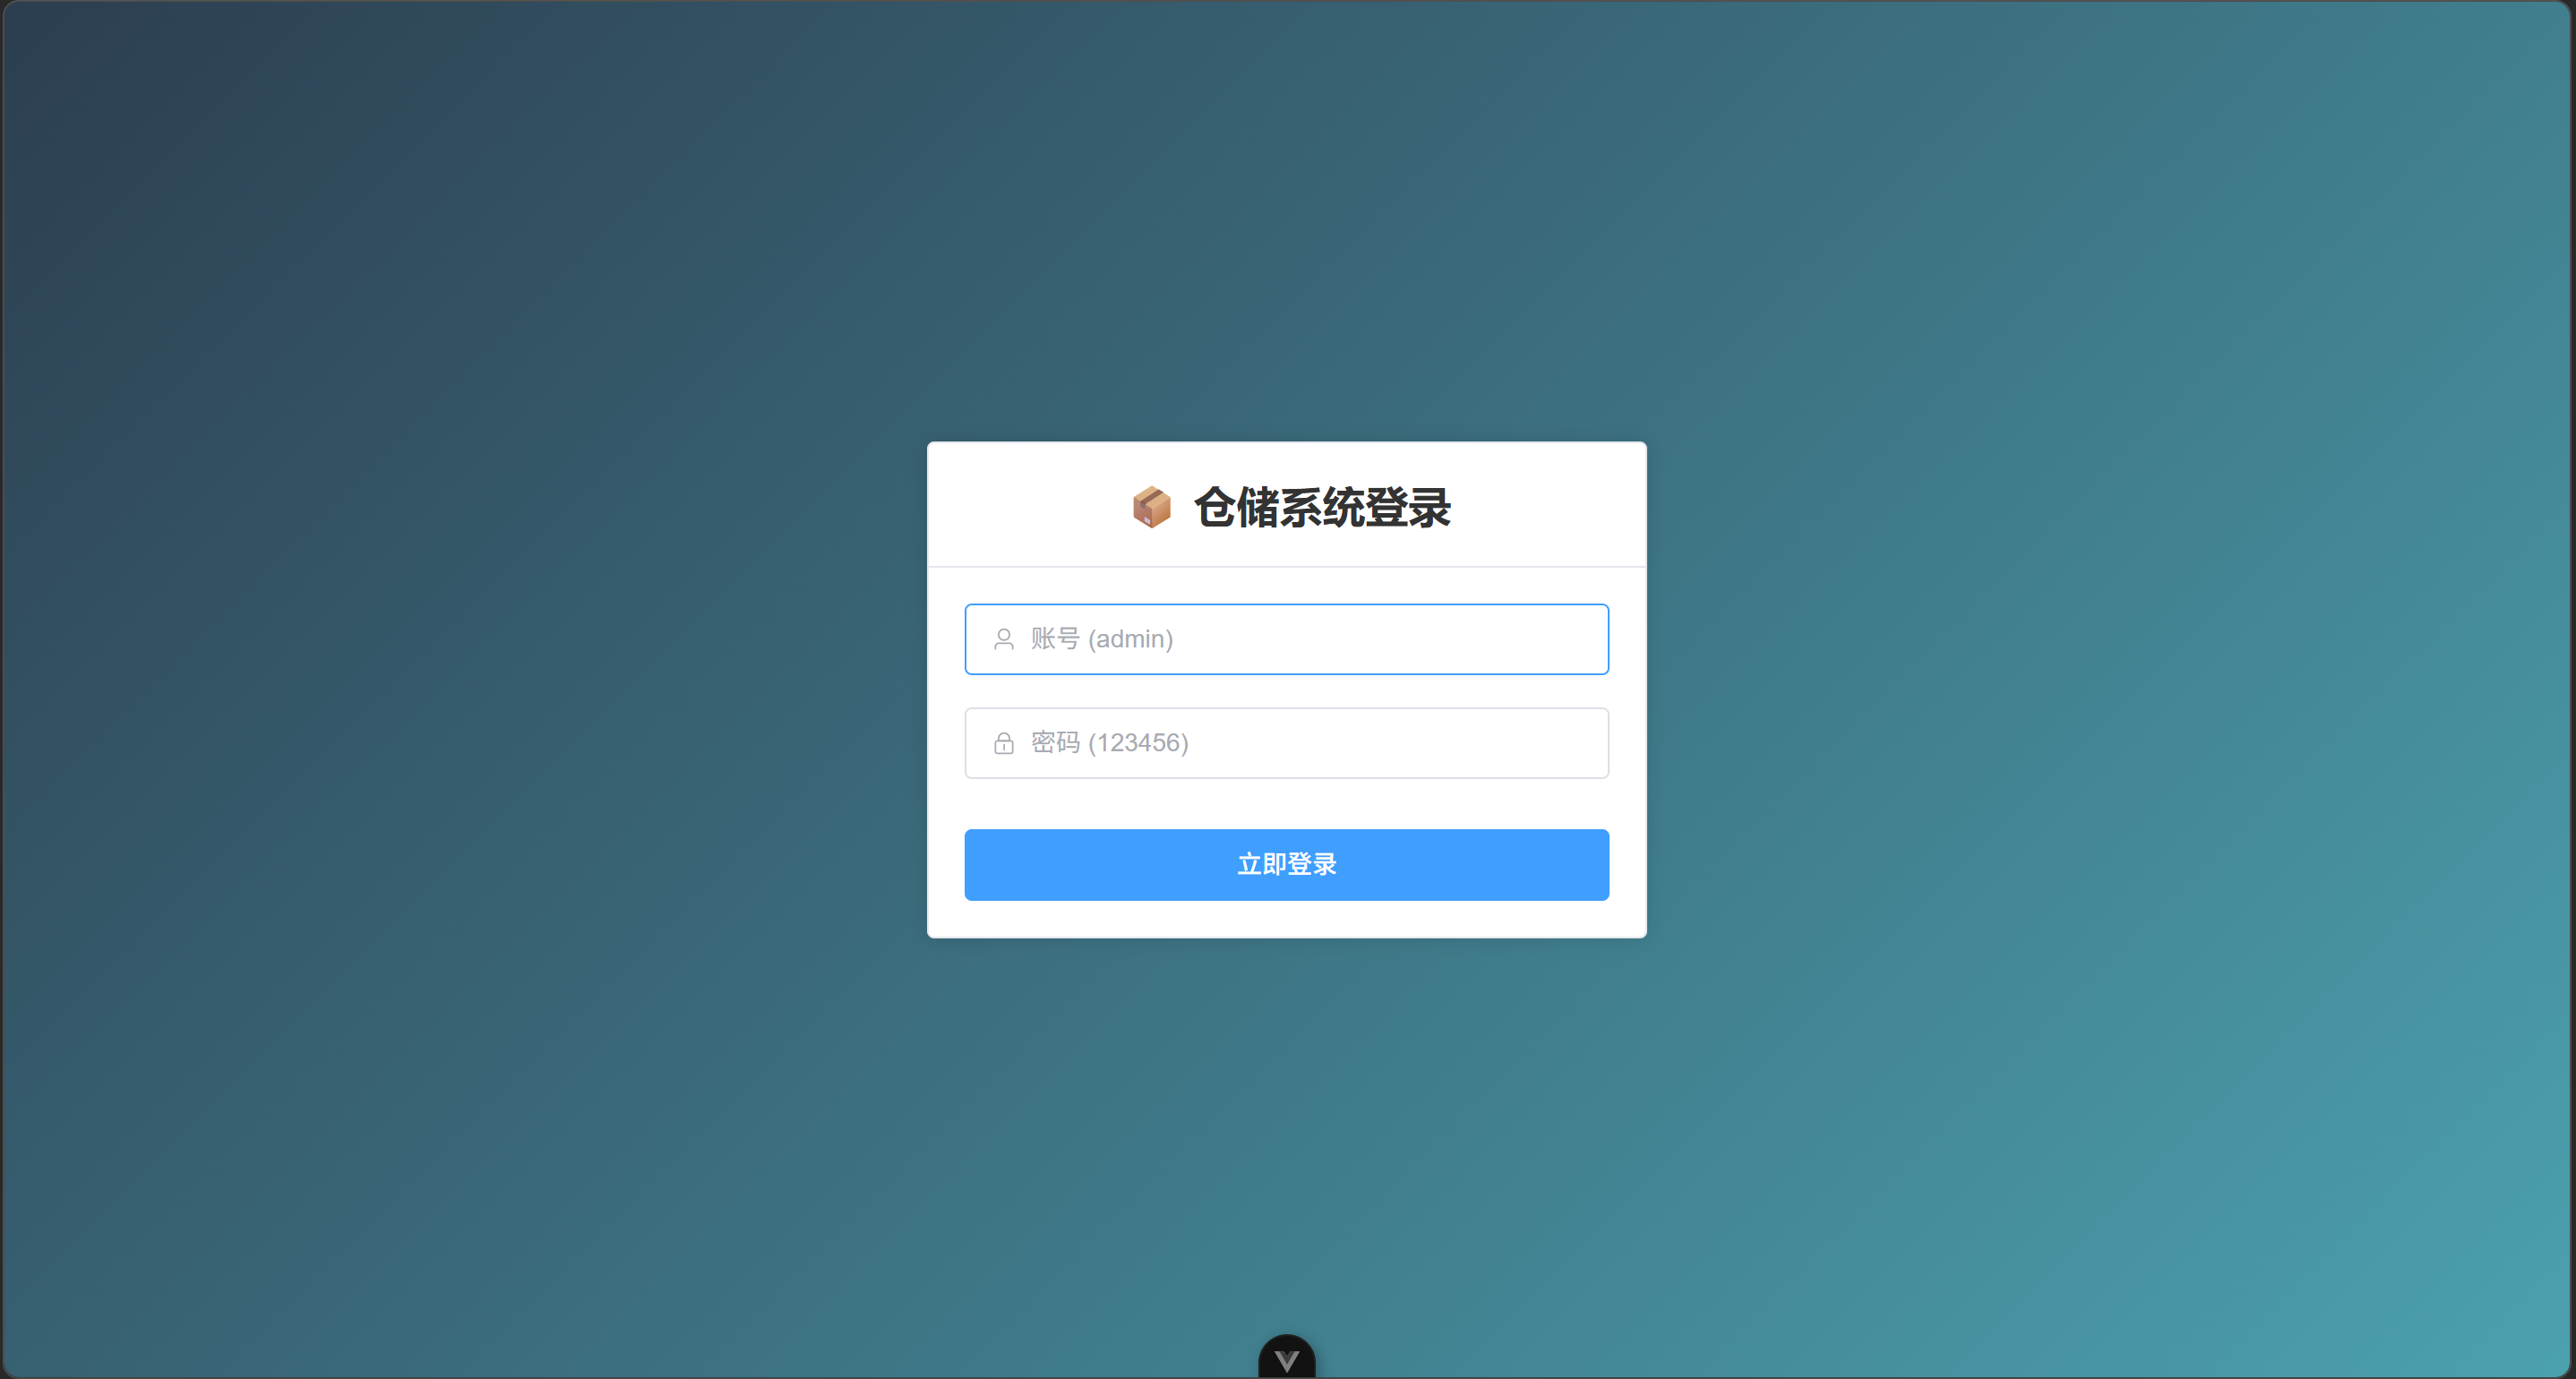
\includegraphics[width=0.8\textwidth]{login.png} 
    \caption{系统登录页}
\end{figure}

\subsection{系统工作台}
登录成功后进入工作台，左侧为导航，右上方展示用户信息。
\begin{figure}[H]
    \centering
    % 请确保图片 dashboard.png 存在于同级目录
    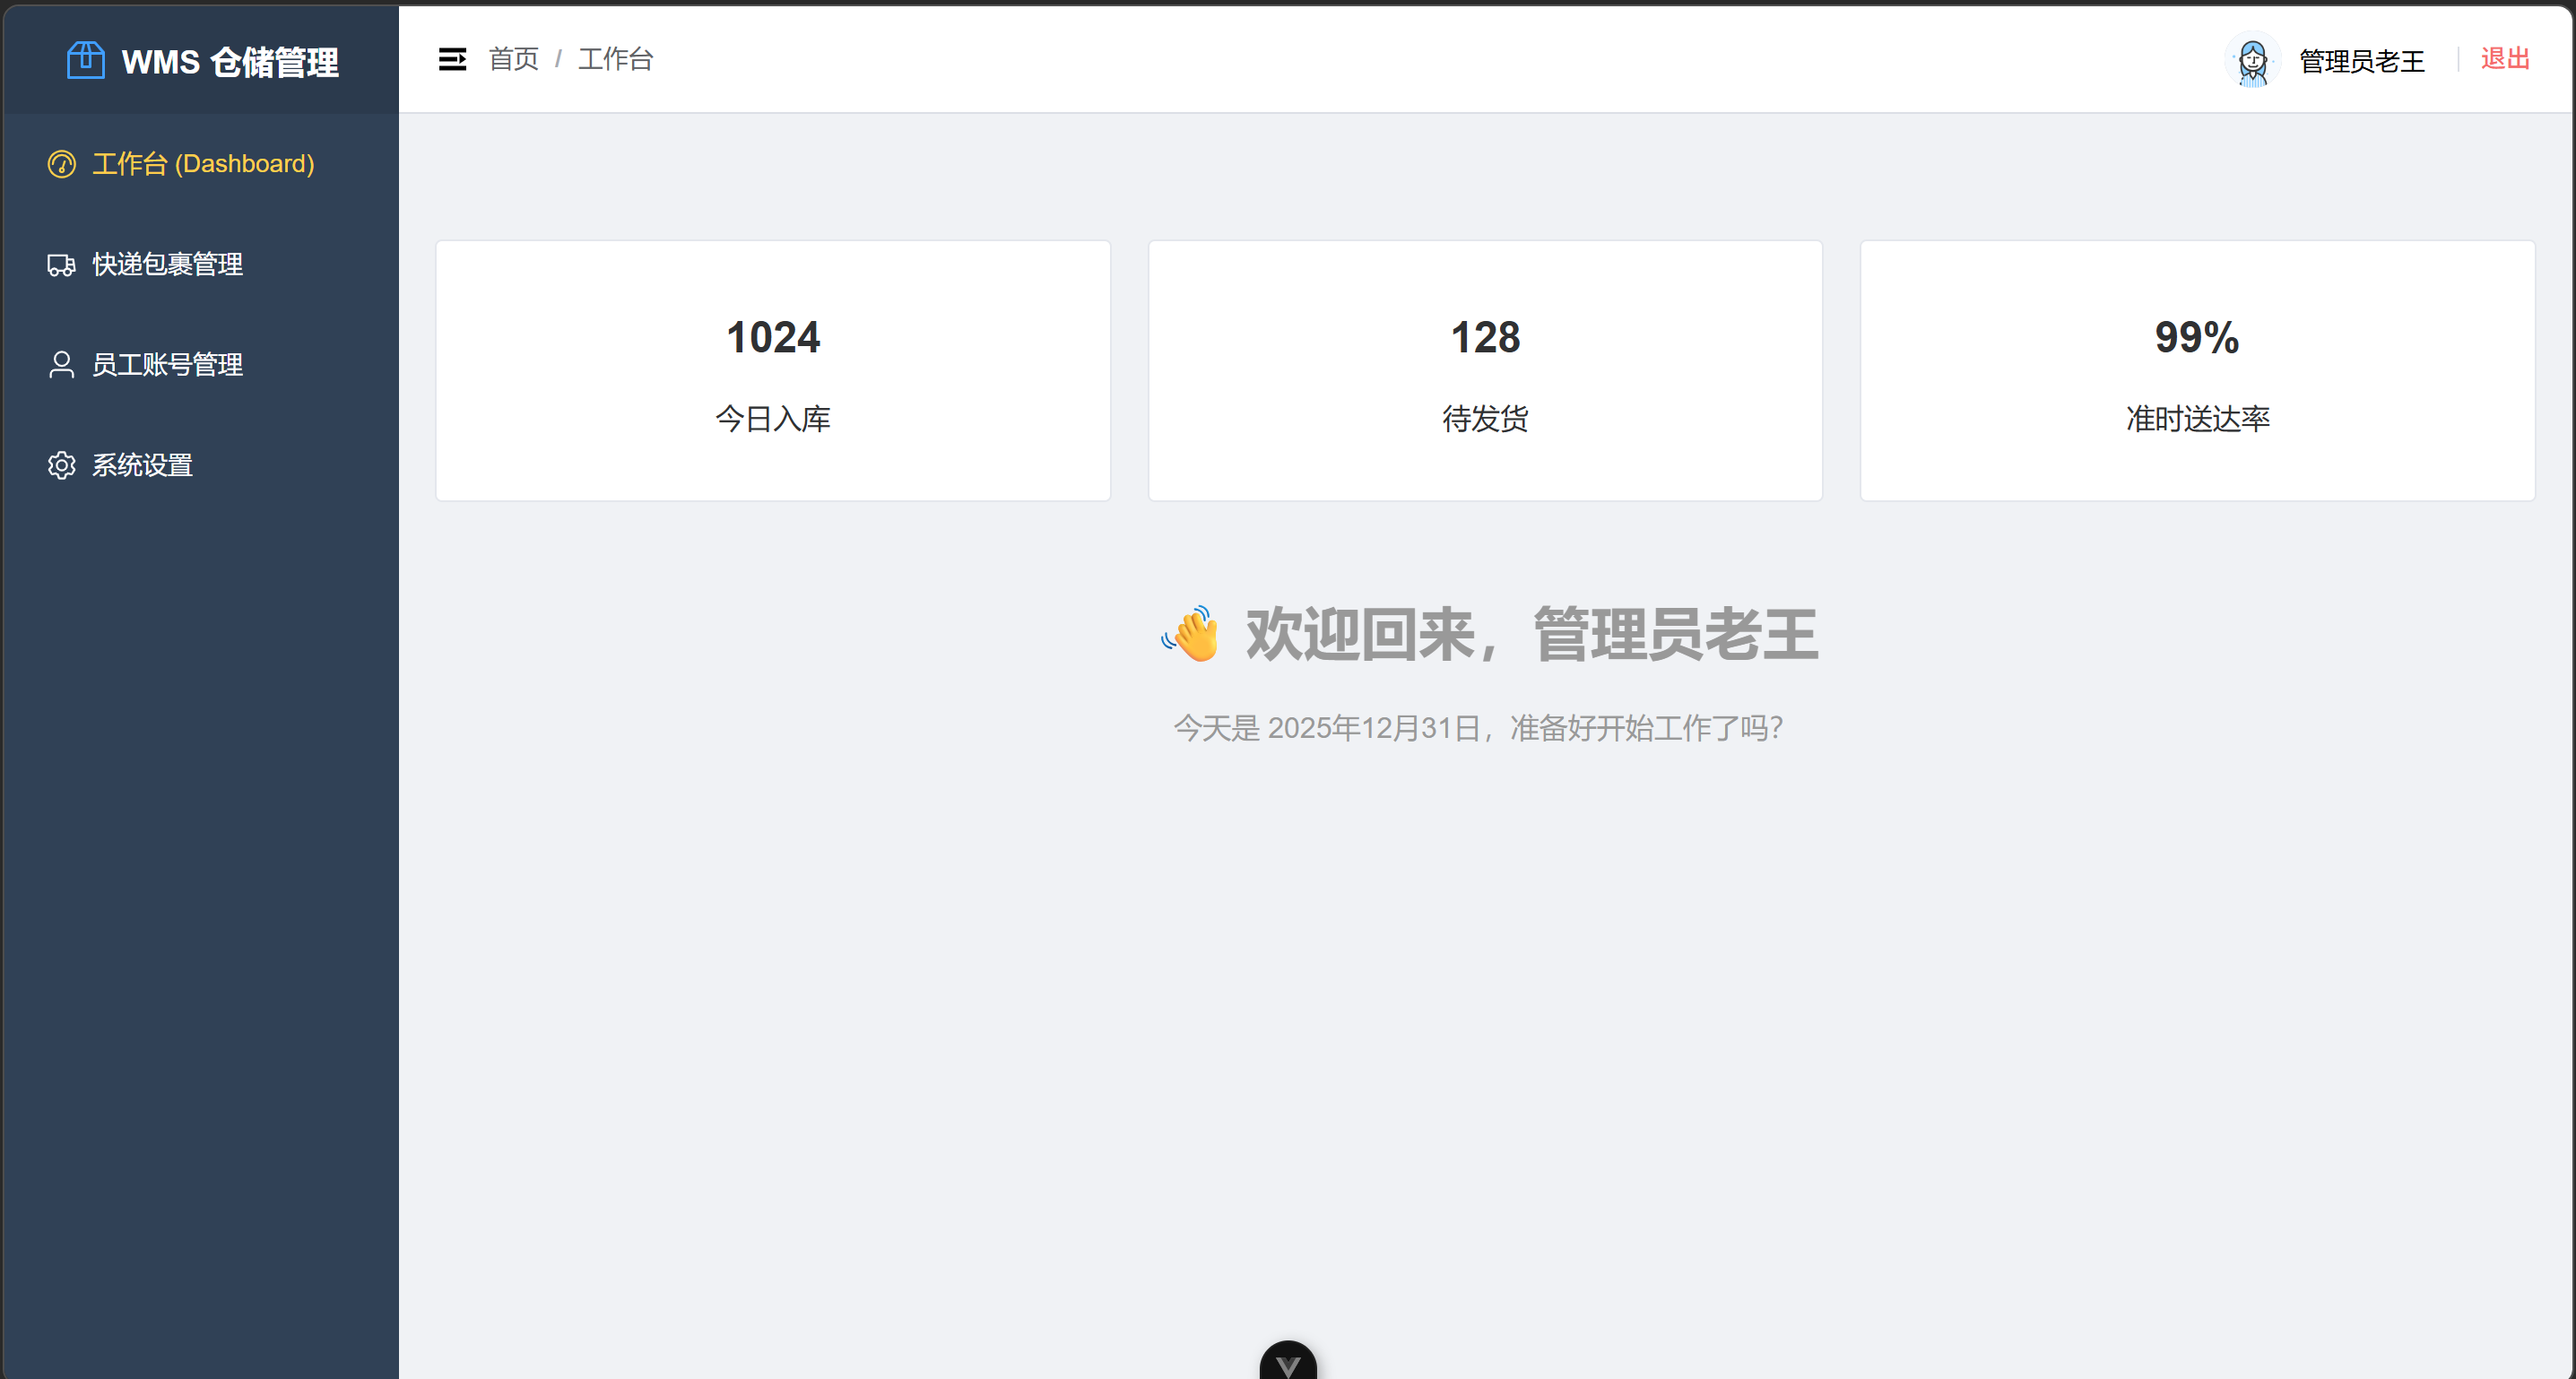
\includegraphics[width=0.8\textwidth]{dashboard.png}
    \caption{管理后台工作台}
\end{figure}

\subsection{包裹管理与新增}
支持通过弹窗新增包裹，并在表格中实时显示物流状态。
\begin{figure}[H]
    \centering
    % 请确保图片 list.png 存在于同级目录
    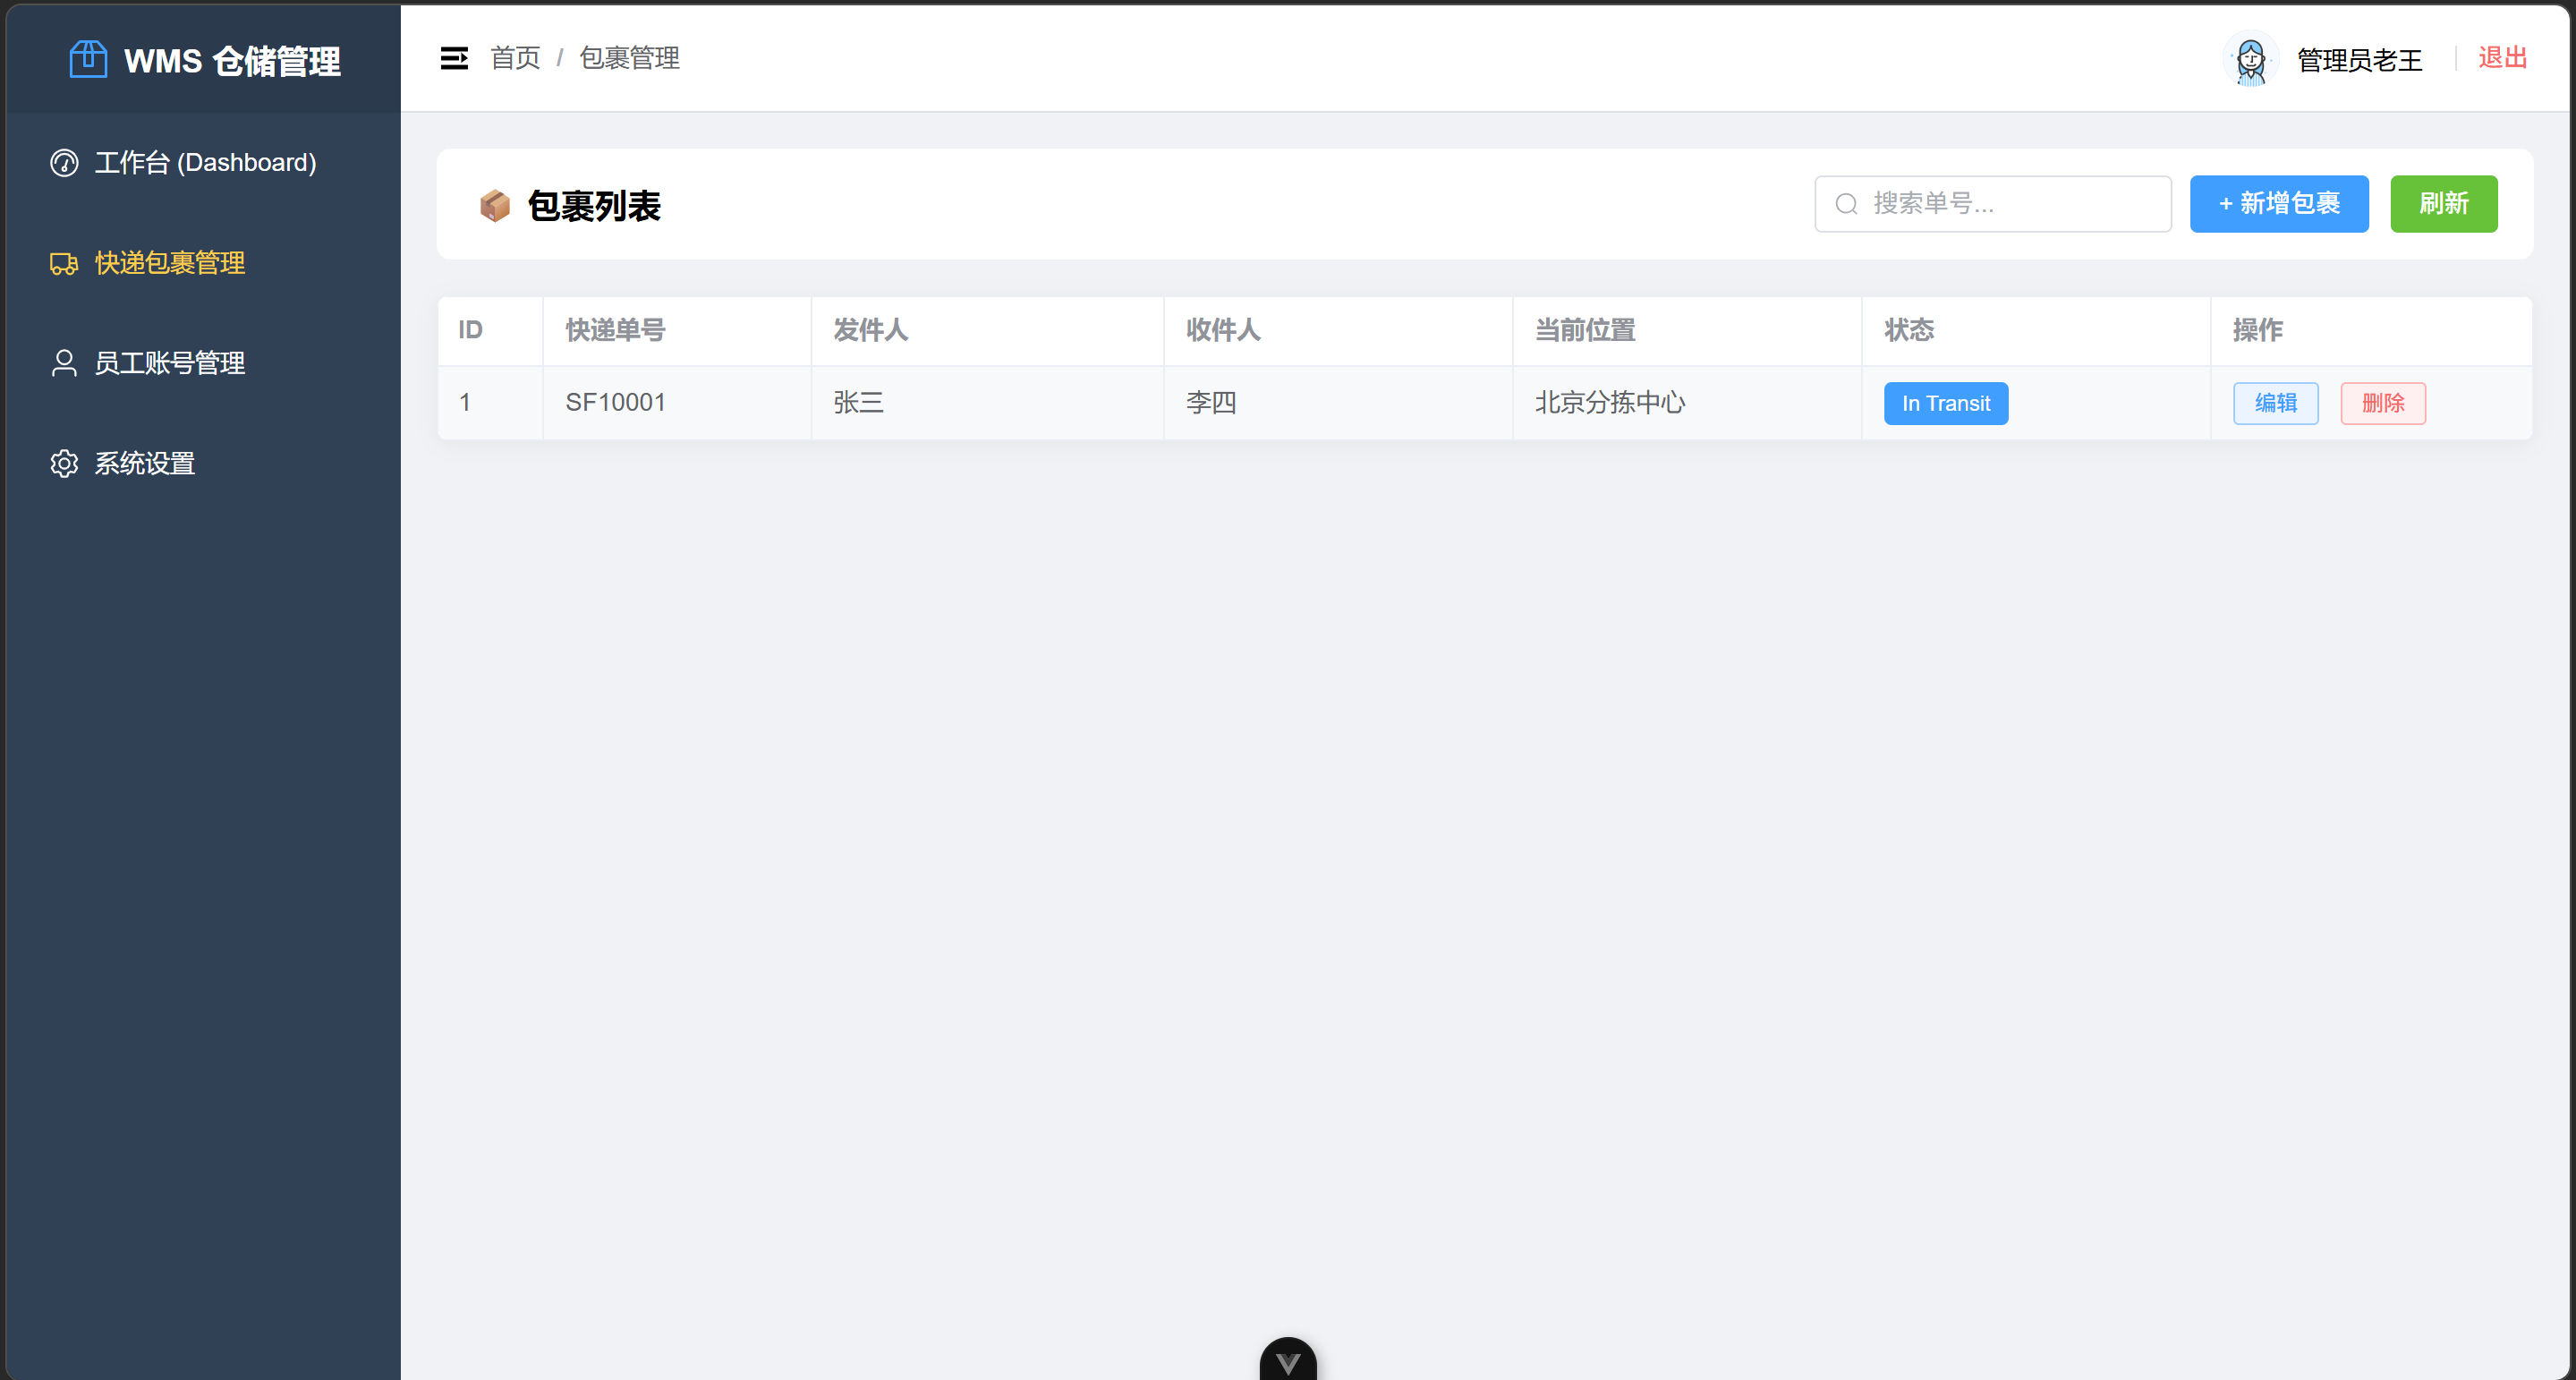
\includegraphics[width=0.8\textwidth]{list.png}
    \caption{增删改查功能演示}
\end{figure}

\section{系统测试分析}

\begin{enumerate}
    \item \textbf{连通性测试}：后端控制台显示 `Connected`，且前端能从数据库拉取到 `Users` 表中的 `admin` 账号信息，登录跳转功能正常。
    \item \textbf{CRUD 业务测试}：
    \begin{itemize}
        \item \textbf{增}：点击“新增包裹”，填写表单后，数据库 `Packages` 表增加一行记录。
        \item \textbf{删}：点击“删除”按钮，前端列表行消失，数据库记录同步被物理删除。
        \item \textbf{改}：更新状态为“已送达”，前端标签颜色变为绿色，状态同步成功。
    \end{itemize}
    \item \textbf{异常测试}：关闭后端服务时，前端弹出“无法连接后端”的红色错误提示，系统健壮性符合预期。
\end{enumerate}

\section{课题收获总结}

\subsection{企业级项目构建体会}
通过本次课程设计，我从零搭建了一个全栈 WMS 系统。最大的体会在于“规范性”：使用 Element Plus 让我明白统一 UI 风格的重要性；使用 SQL Server 让我体会到了关系型数据库在企业数据存储中的核心地位。

\subsection{解决问题的感悟}
开发过程中最大的困难是 Node.js 连接本地 SQL Server 时的证书与驱动问题。通过查阅文档，我学会了使用 `msnodesqlv8` 配合 `ODBC Driver 17` 来解决 Windows 身份验证问题。这让我明白，全栈开发不仅是写代码，更是环境配置与调试能力的考验。

\section{参考文献}
\begin{enumerate}[label={[\arabic*]}]
    \item Vue.js 3.0 官方文档. \url{https://vuejs.org/}
    \item Element Plus 组件库指南. \url{https://element-plus.org/}
    \item Microsoft SQL Server 连接驱动文档. \url{https://www.npmjs.com/package/mssql}
\end{enumerate}

\end{document}